
\documentclass[11pt]{exam} % https://www.ctan.org/pkg/exam?lang=en

\usepackage[lmargin=1.in,rmargin=1.in,tmargin=1.in,bmargin=1in]{geometry}
\usepackage{setspace}
\usepackage[pdftex]{graphicx}
\usepackage{titling}
\usepackage[
	pdfauthor={Brian Weinstein},
	pdftitle={Homework 1},
	bookmarks=true,
	colorlinks=true,
	linkcolor=blue,
	urlcolor=blue,
	citecolor=blue,
	pdftex,
	linktocpage=true
	]{hyperref}
\usepackage[textsize=tiny]{todonotes}
\usepackage{float}
\setlength\parindent{0pt}
\usepackage{lipsum}
\usepackage{amsmath}
\usepackage{caption}


\qformat{\textbf{Problem \thequestion: \thequestiontitle}\quad \hfill}


\pagestyle{headandfoot}
\runningheadrule
\firstpageheader{}{}{}
\runningheader{\theauthor}{\thetitle}{\thedate}
\firstpagefooter{}{\thepage}{}
\runningfooter{}{\thepage}{}


\usepackage{xcolor}
\usepackage{adjustbox}
\usepackage{verbatim}
\definecolor{shadecolor}{rgb}{.9, .9, .9}

\newenvironment{code}%
   {\par\noindent\adjustbox{margin=1ex,bgcolor=shadecolor,margin=0ex \medskipamount}\bgroup\minipage\linewidth\verbatim}%
   {\endverbatim\endminipage\egroup}

\newenvironment{codeSmall}%
   {\par\noindent\adjustbox{margin=1ex,bgcolor=shadecolor,margin=0ex \medskipamount}\bgroup\minipage\linewidth\verbatim\footnotesize}%
   {\endverbatim\endminipage\egroup}

\newcommand{\ramsey}{\href{http://www.statisticalsleuth.com/}{Ramsey }}



\begin{document}


\title{STAT W4201 001, Homework 5}
\author{Brian Weinstein (bmw2148)}
\date{March 2, 2016}
\maketitle

Code is attached here and also posted at \href{https://github.com/BrianWeinstein/advanced-data-analysis}{https://github.com/BrianWeinstein/advanced-data-analysis}. Where relevant, code snippets and output are are included in-line.

\begin{questions}


\titledquestion{\ramsey 7.18}

\begin{parts}

\part \textit{Find the standard error of prediction for the prediction of pH at 5 hours after slaughter.}

The calculations in Display 7.12 give us $\hat{\beta}_0=6.9836$, $\hat{\beta}_1=-0.7257$, $\hat{\sigma}=0.08226$, $n=10$, $\overline{X}=1.190$, $s_X^2=0.6344$.

Therefore, the standard error of prediction for the pH at 5 hours is
\begin{align*}
\text{SE}\left[ \text{Pred}\{ Y | X_0=\log(5)=1.609438  \} \right] &= \hat{\sigma} \sqrt{ 1 + \frac{1}{n} + \frac{(X_0 - \overline{X})^2}{(n-1)s_X^2} } \\
&= (0.08226) \sqrt{ 1 + \frac{1}{10} + \frac{(1.609438 - 1.190)^2}{9 \cdot 0.6344} } \\
&= 0.0875
\end{align*}


\part \textit{Construct a 95\% prediction interval at 5 hours after slaughter.}

The prediction of pH level at 5 hours is,
\begin{align*}
{Pred}\{ Y | X_0=\log(5)=1.609438  \}  &=  \beta_0 + \beta_1 \cdot \log(5) \\
&= 6.9836 - 0.7257 \cdot 1.609438 \\
&= 5.8156.
\end{align*}

A 95\% prediction confidence interval at 5 hours is given by
\begin{gather*}
5.8156 \pm t_{8}(0.975) \cdot \text{SE}\left[ \text{Pred}\{ Y | X_0=\log(5) \} \right] \\
5.8156 \pm 2.3060 \cdot 0.0875 \\
5.8156 \pm 0.2017 \\
\Rightarrow [5.6139, 6.0173].
\end{gather*}


\end{parts}


\titledquestion{\ramsey 7.24}

\begin{parts}

\part \textit{With a statistical computer package and the data in the file ex0724, obtain the least squares fits to the four simple regressions, individually, to confirm the estimates and standard errors presented in Display 7.17.}

Confirming the estimates and standard errors from Display 7.17:

\begin{subparts}

\subpart Denmark
\begin{codeSmall}
> lmDenmark <- lm(formula=Denmark~Year, data=birthData)
> summary(lmDenmark)$coefficients
                  Estimate   Std. Error   t value     Pr(>|t|)
(Intercept)  0.59872329381 0.0408047207 14.672893 2.395722e-18
Year        -0.00004288538 0.0000206916 -2.072598 4.423828e-02
\end{codeSmall}$

\subpart The Netherlands
\begin{codeSmall}
> lmNetherlands <- lm(formula=Netherlands~Year, data=birthData)
> summary(lmNetherlands)$coefficients
                  Estimate   Std. Error   t value     Pr(>|t|)
(Intercept)  0.67239837505 0.0279195810 24.083398 1.365923e-26
Year        -0.00008084321 0.0000141577 -5.710196 9.636921e-07
\end{codeSmall}$

\subpart Canada
\begin{codeSmall}
> lmCanada <- lm(formula=Canada~Year, data=birthData)
> summary(lmCanada)$coefficients
                 Estimate    Std. Error   t value     Pr(>|t|)
(Intercept)  0.7337857143 0.05480068278 13.390083 3.983523e-11
Year        -0.0001111688 0.00002767698 -4.016653 7.375947e-04
\end{codeSmall}$

\subpart United States
\begin{codeSmall}
> lmUsa <- lm(formula=USA~Year, data=birthData)
> summary(lmUsa)$coefficients
                  Estimate     Std. Error   t value     Pr(>|t|)
(Intercept)  0.62008571429 0.018598766807 33.340152 2.523643e-18
Year        -0.00005428571 0.000009393273 -5.779212 1.439109e-05
\end{codeSmall}$

\end{subparts}

\part \textit{Obtain the t-statistic for the test that the slopes of the regressions are zero, for each of the four countries. Is there evidence that the proportion of male births is truly declining?}

The t-statistics and associated two-sided p-values are computed and shown in the output of part (a). For the \texttt{Year} variable:

\begin{subparts}

\subpart Denmark

The t-statistic is $-2.0726$, with a one-sided p-value of $0.0221$. The data provides moderate, but not convincing evidence, that the proportion of male births is truly declining in Denmark.


\subpart The Netherlands

The t-statistic is $-5.7102$, with a one-sided p-value of $0.000000482$. The data provides overwhelming evidence that the proportion of male births is truly declining in the Netherlands.


\subpart Canada

The t-statistic is $-4.0167$, with a one-sided p-value of $0.000369$. The data provides convincing evidence that the proportion of male births is truly declining in Canada.


\subpart United States

The t-statistic is $-5.7792$, with a one-sided p-value of $0.00000720$. The data provides overwhelming evidence that the proportion of male births is truly declining in the United States.

\end{subparts}


\part \textit{Explain why the United States can have the largest of the four t-statistics (in absolute value) even though its slope is only the third largest (in absolute value).}

In the hypothesis that the slopes of the regressions are zero, the t-statistic is defined as $Estimate/\text{SE}(Estimate)$. So even though the slope is only the third largest (in absolute value), the standard error on the estimate is small enough to make the $Estimate/\text{SE}(Estimate)$ ratio largest for the USA.

\part \textit{Explain why the standard error of the estimated slope is smaller for the United States than for Canada, even though the sample size is the same.}

The standard error of the estimated slope is given by
$$\text{SE}(\hat{\beta}_1) = \hat{\sigma} \sqrt{\frac{1}{(n-1)s_X^2}},$$
where $s_X^2$ is the sample variance of the $X$'s.

For the US and Canada, $n$ and $s_X^2$ are the same (it's the same sample size, using the same subset of years), but $\hat{\sigma}$ is different.

$$\hat{\sigma} = \sqrt{\frac{\text{RSS}_j}{\text{Degrees of freedom}}} = \sqrt{\frac{\text{RSS}_j}{n-2}} = \sqrt{\frac{\text{RSS}_j}{19}},$$

where $\text{RSS}_j$ is the sum of squared residuals for group j.

For the US, the RSS is
\begin{codeSmall}
> sum((lmUsa$residuals)^2)
[1] 0.000001290857
\end{codeSmall}$

and for Canada, the RSS is
\begin{codeSmall}
> sum((lmCanada$residuals)^2)
[1] 0.00001120681
\end{codeSmall}$

Since the RSS for the US model is an order of magnitude smaller than the RSS for the Canada model (and since all other parameters in $\text{SE}(\hat{\beta}_1)$ are identical) the standard error for the estimated slope is smaller for the US.

\part \textit{Can you think of any reason why the standard deviations about the regression line might be different for the four countries? (Hint: The proportion of males is a kind of average, i.e., the average number of births that are male.)}

There's no reason to think that the standard deviations about the regression lines would be the same for the four countries. These are samples from four different populations, and there's no reason to think their sampling distributions will have identical spreads.


\end{parts}



\titledquestion{\ramsey 7.28}

\begin{parts}

\part \textit{Is the neuron activity different in the stringed musicians and the controls?}

A boxplot of the neuronal activity index for the two groups is shown in Figure \ref{fig:3_orig}.

\begin{figure}[!h]
	\centering
	\captionsetup{width=0.8\textwidth}
	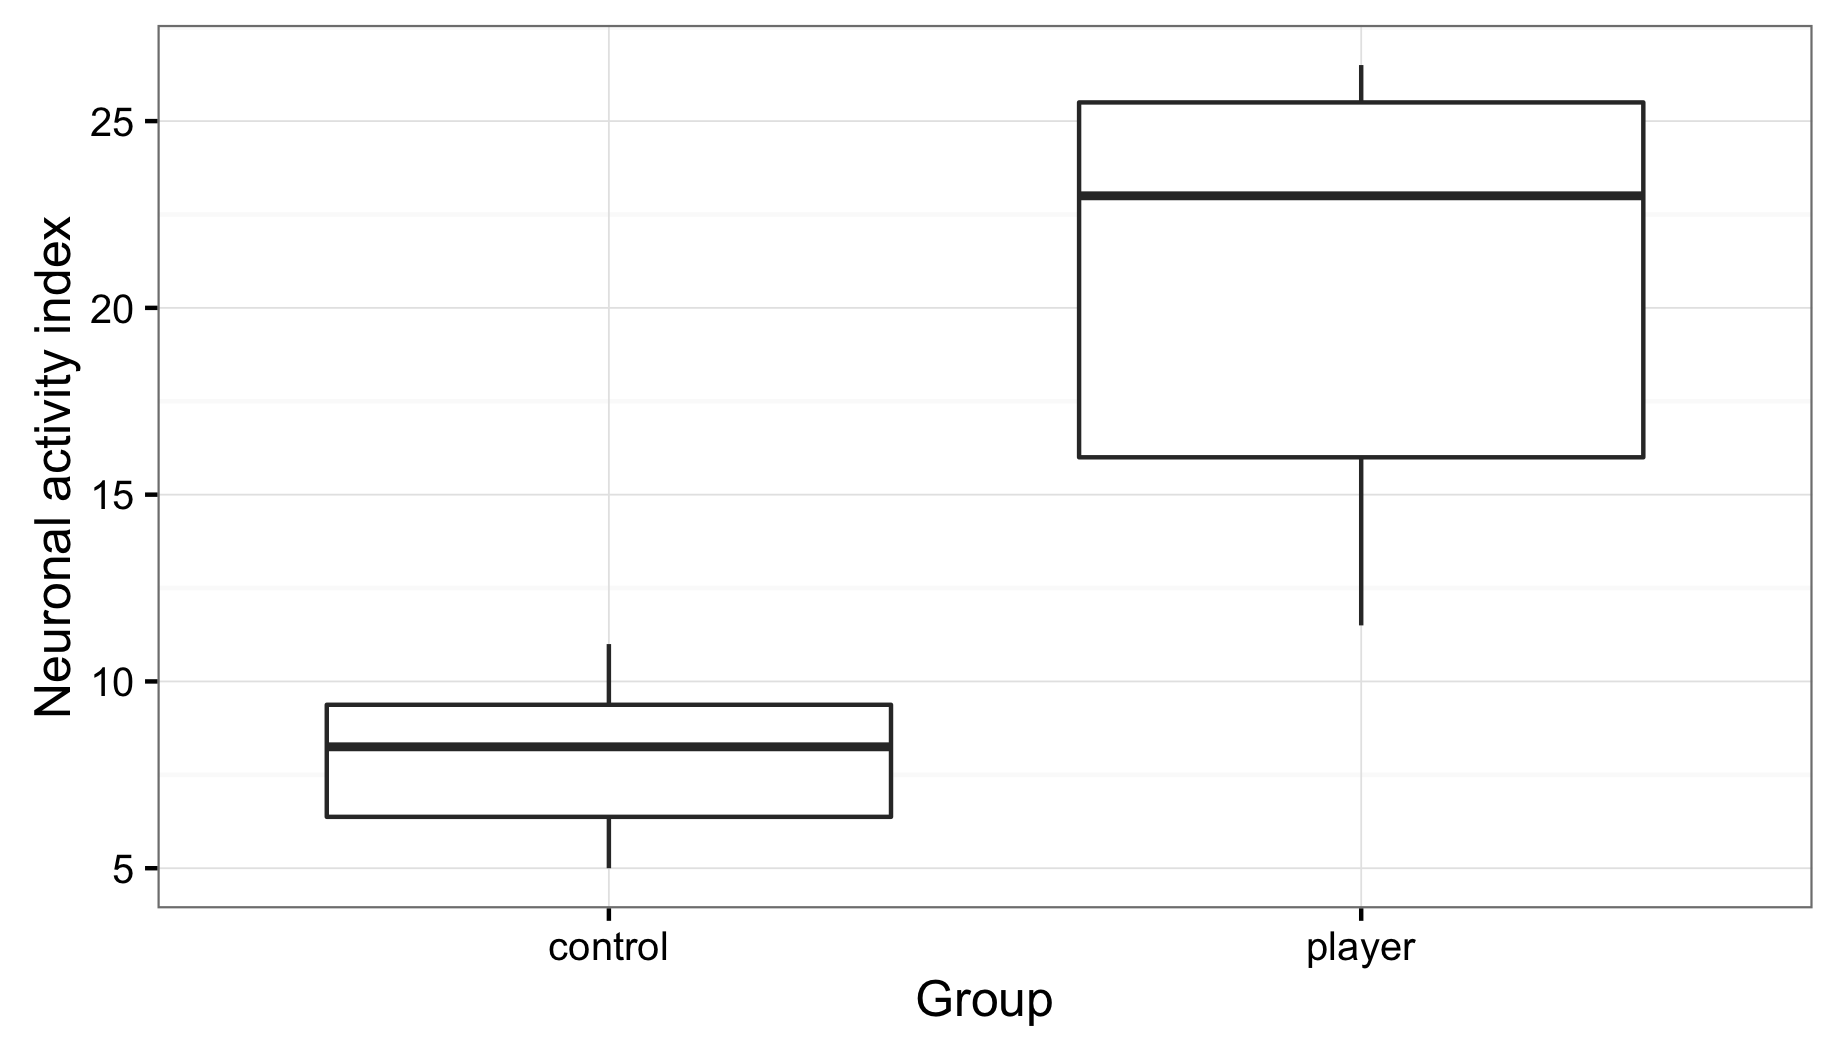
\includegraphics[width=4.25in]{3_orig.png}
	\caption{Boxplots of neuronal activity index (D5 dipole strength, in nA-m) for a groups of string players (player) and a group of non-string players (control).}
	\label{fig:3_orig}
\end{figure}

The two groups have unequal variances. On the log scale, however, the variances are nearly equal, as shown below and in Figure \ref{fig:3_log}.

\begin{codeSmall}
> # compare group standard deviations on the original and log scales
> brainData %>%
+   group_by(Group) %>%
+   summarize(sd(Activity), sd(LogActivity)) %>%
+   as.data.frame()
    Group sd(Activity) sd(LogActivity)
1 control     2.258318       0.2983304
2  player     5.588928       0.2976929
\end{codeSmall}

\begin{figure}[!h]
	\centering
	\captionsetup{width=0.8\textwidth}
	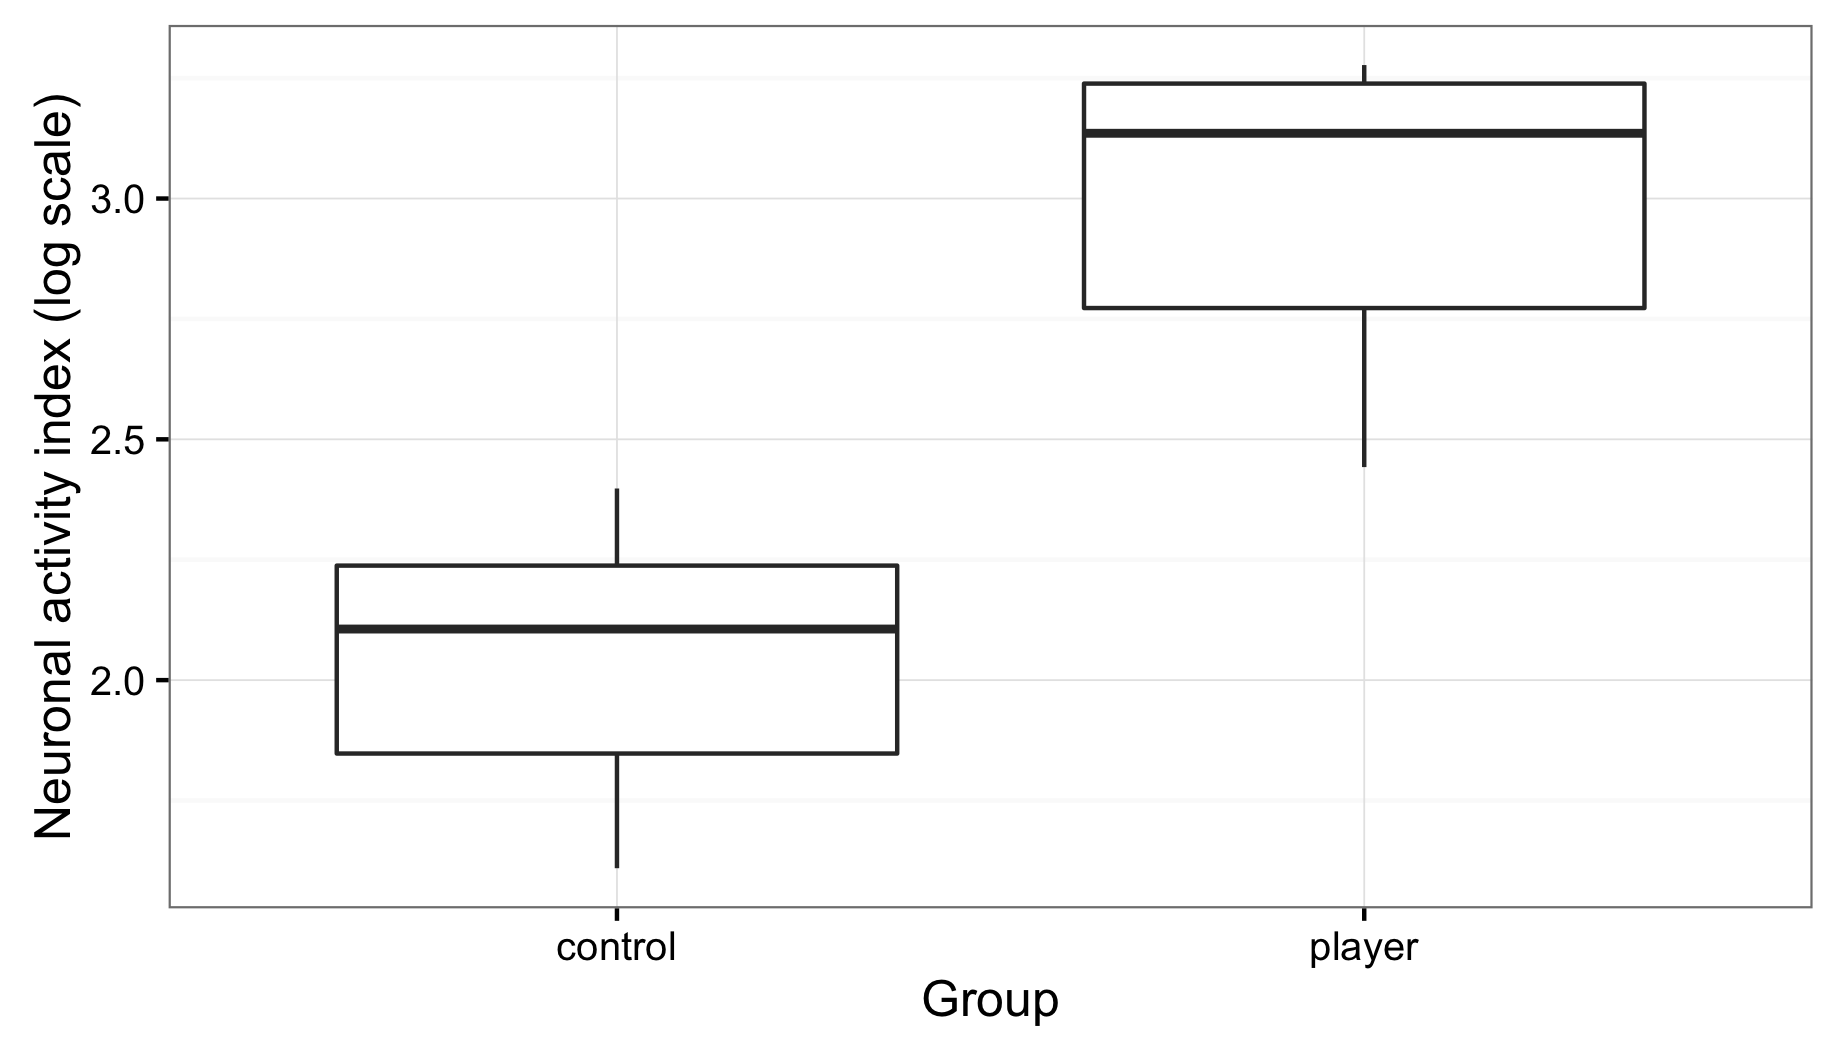
\includegraphics[width=4.25in]{3_log.png}
	\caption{Boxplots of neuronal activity index (D5 dipole strength, in log(nA-m)) for a groups of string players (player) and a group of non-string players (control).}
	\label{fig:3_log}
\end{figure}


Using a two-sample t-test on the log-transformed neuronal activity index, we find overwhelming evidence that mean log activities are not equal in the two groups on the log scale (two-sided p-value: $0.00004312$). Back-transforming the estimate and confidence interval from the log scale to the original scale, it's estimated that the mean neuronal activity index is $2.5731$ times higher for the group of string players than the group of non-string players (95\% confidence interval: $1.8329$ to $3.6123$ times).


\part \textit{Is the amount of activity associated with the number of years the individual has been playing the instrument?}

This is equivalent to testing if $\hat{\beta}_1 \neq 0$ in the linear regression of $\hat{\mu}\{Y|X\}=\hat{\beta}_0 + \hat{\beta}_1 X$, where $Y$ is the neuronal activity index and $X$ is the number of years an individual has been playing the instrument. The coefficients of the linear regression are shown below, and a plot of Years vs Activity is shown in Figure \ref{fig:3b_fit}. The residual plot of the fitted model is shown in Figure \ref{fig:3b_resid}.


\begin{codeSmall}
> lmBrain <- lm(formula=Activity~Years, data=brainData)
> summary(lmBrain)$coefficients
             Estimate Std. Error  t value        Pr(>|t|)
(Intercept) 8.3872549  1.1148871 7.522963 0.0000043546830
Years       0.9971405  0.1110454 8.979574 0.0000006178311
\end{codeSmall}$

The data provides overwhelming evidence that the amount of neuronal activity is associated with the number of years the individual has been playing the instrument. The slope of the regression line is estimated to be $\hat{\beta}_1 = 0.9971$, with a two-sided p-value (for the test that $\beta_1 = 0$) of $6.178 \times 10^{-7}$.

\begin{figure}[!h]
	\centering
	\captionsetup{width=0.8\textwidth}
	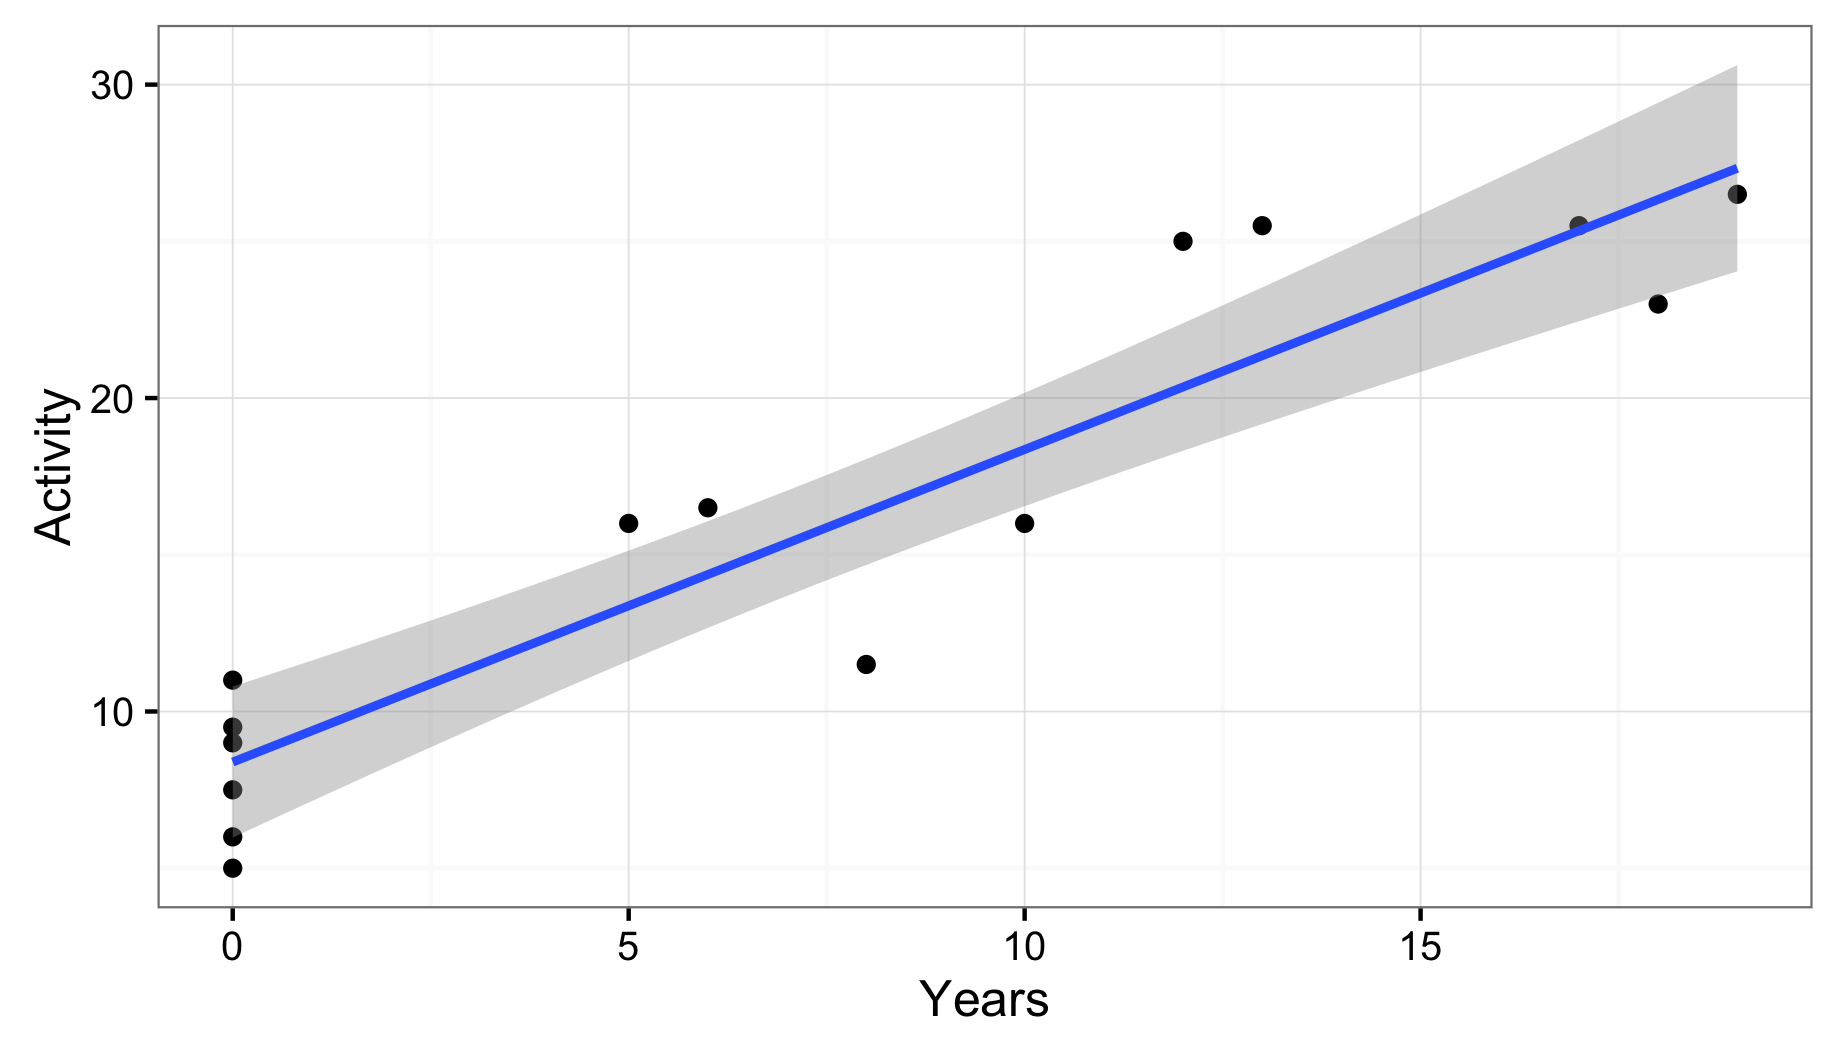
\includegraphics[width=4.25in]{3b_fit.png}
	\caption{Scatterplot and linear regression of Activity vs Years. A 95\% confidence band for the entire regression line is shown in gray.}
	\label{fig:3b_fit}
\end{figure}

\begin{figure}[!h]
	\centering
	\captionsetup{width=0.8\textwidth}
	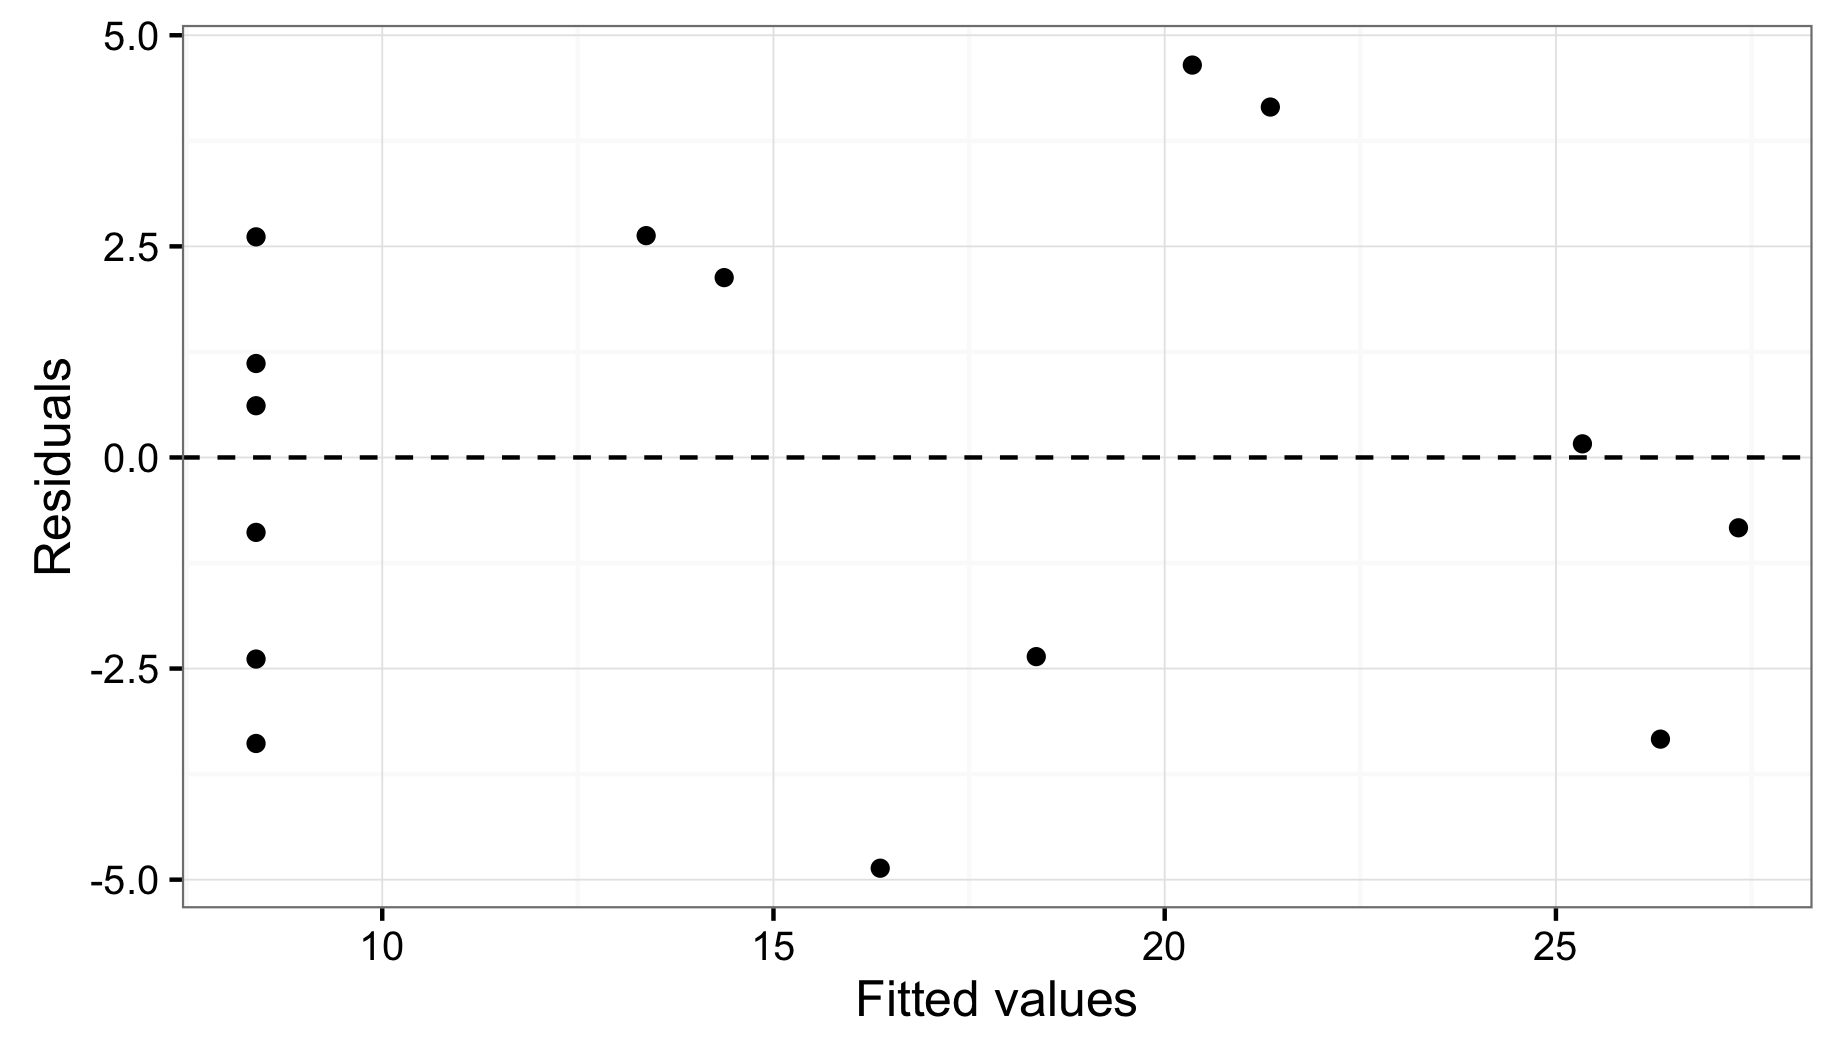
\includegraphics[width=4.25in]{3b_resid.png}
	\caption{Residual plot for the fitted model from Figure \ref{fig:3b_fit}.}
	\label{fig:3b_resid}
\end{figure}


\end{parts}



\titledquestion{\ramsey 8.17}

\begin{parts}

\part \textit{Use scatterplots of the raw data, along with trial and error, to determine transformations of $Y=\text{Ragwort dry mass}$ and of $X=\text{Flea beetle load}$ that will produce an approximate linear relationship.}

Scatterplots of the raw data and 3 log transformations of the data are shown in Figure \ref{fig:4a}. For ease of interpretation, I only examined log-transformed variables.

\begin{figure}[!h]
	\centering
	\captionsetup{width=0.8\textwidth}
	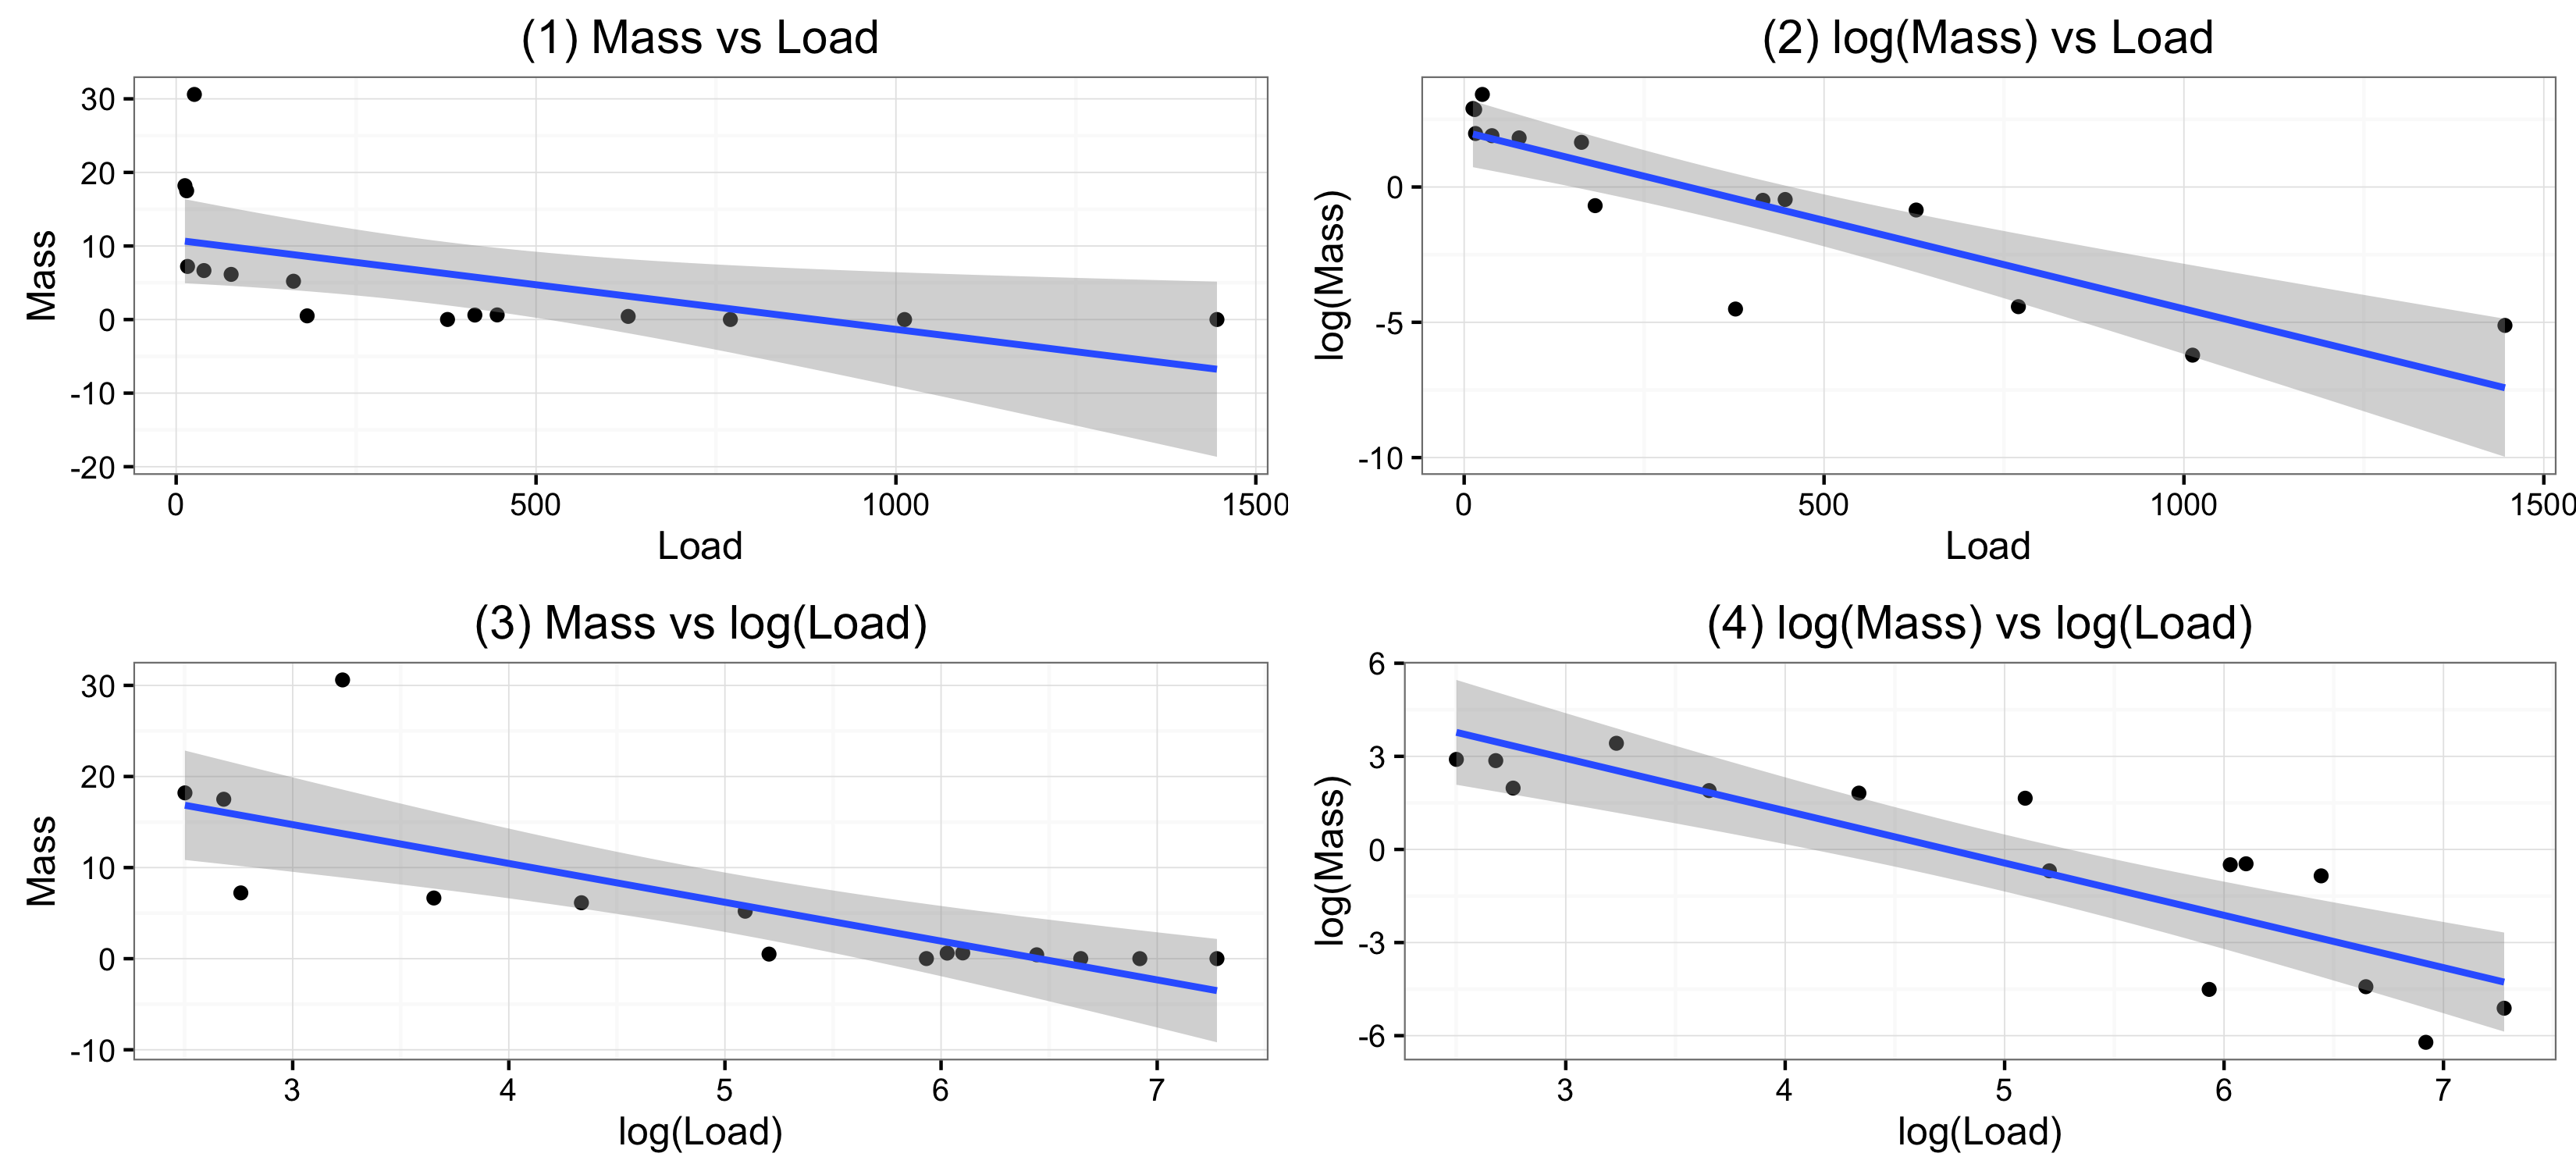
\includegraphics[width=\textwidth]{4a.png}
	\caption{Scatterplots of the raw data and 3 log transformations of the data.}
	\label{fig:4a}
\end{figure}

Log-transforming both the response (Mass) and explanatory variables (Load) produces an approximately linear relationship.

\part \textit{Fit a linear regression model on the transformed scale; calculate residuals and fitted values.} \label{prob:0817b}
Using the \texttt{lm} R function, a linear regression of log(Mass) on log(Load) is shown below.

\begin{codeSmall}
> lmPest <- lm(formula=LogMass~LogLoad, data=pestData)
> summary(lmPest)

Call:
lm(formula = LogMass ~ LogLoad, data = pestData)

Residuals:
     Min       1Q   Median       3Q      Max 
-2.54217 -1.04130  0.06406  1.40544  2.24600 

Coefficients:
            Estimate Std. Error t value  Pr(>|t|)    
(Intercept)    7.988      1.383   5.774 0.0000645 ***
LogLoad       -1.685      0.264  -6.383 0.0000241 ***
---
Signif. codes:  0 ‘***’ 0.001 ‘**’ 0.01 ‘*’ 0.05 ‘.’ 0.1 ‘ ’ 1

Residual standard error: 1.646 on 13 degrees of freedom
Multiple R-squared:  0.7581,	Adjusted R-squared:  0.7395 
F-statistic: 40.74 on 1 and 13 DF,  p-value: 0.00002407
\end{codeSmall}

Residuals and fitted values are shown below.

\begin{codeSmall}
> residuals(lmPest)
          1           2           3           4           5           6           7 
-0.87164605 -0.60823442 -1.36047140  0.87704266  0.06405890  1.13328141  2.24600408 
          8           9          10          11          12          13          14 
 0.09207006  1.67760559  1.82962887  2.01739421 -2.50142865 -1.21096053 -0.84217066 
         15 
-2.54217409 
> 
> fitted(lmPest)
         1          2          3          4          5          6          7          8 
 3.7730676  3.4704353  3.3373263  2.5439574  1.8320606  0.6815433 -0.5954242 -0.7812252 
         9         10         11         12         13         14         15 
-2.1702639 -2.2916643 -2.8683655 -2.0084314 -3.2118881 -4.2738252 -3.6724340 
\end{codeSmall}



\part \textit{Look at the residual plot. Do you want to try other transformations? What do you suggest?}

The residual plot is shown in Figure \ref{fig:4c}.

\begin{figure}[!h]
	\centering
	\captionsetup{width=0.8\textwidth}
	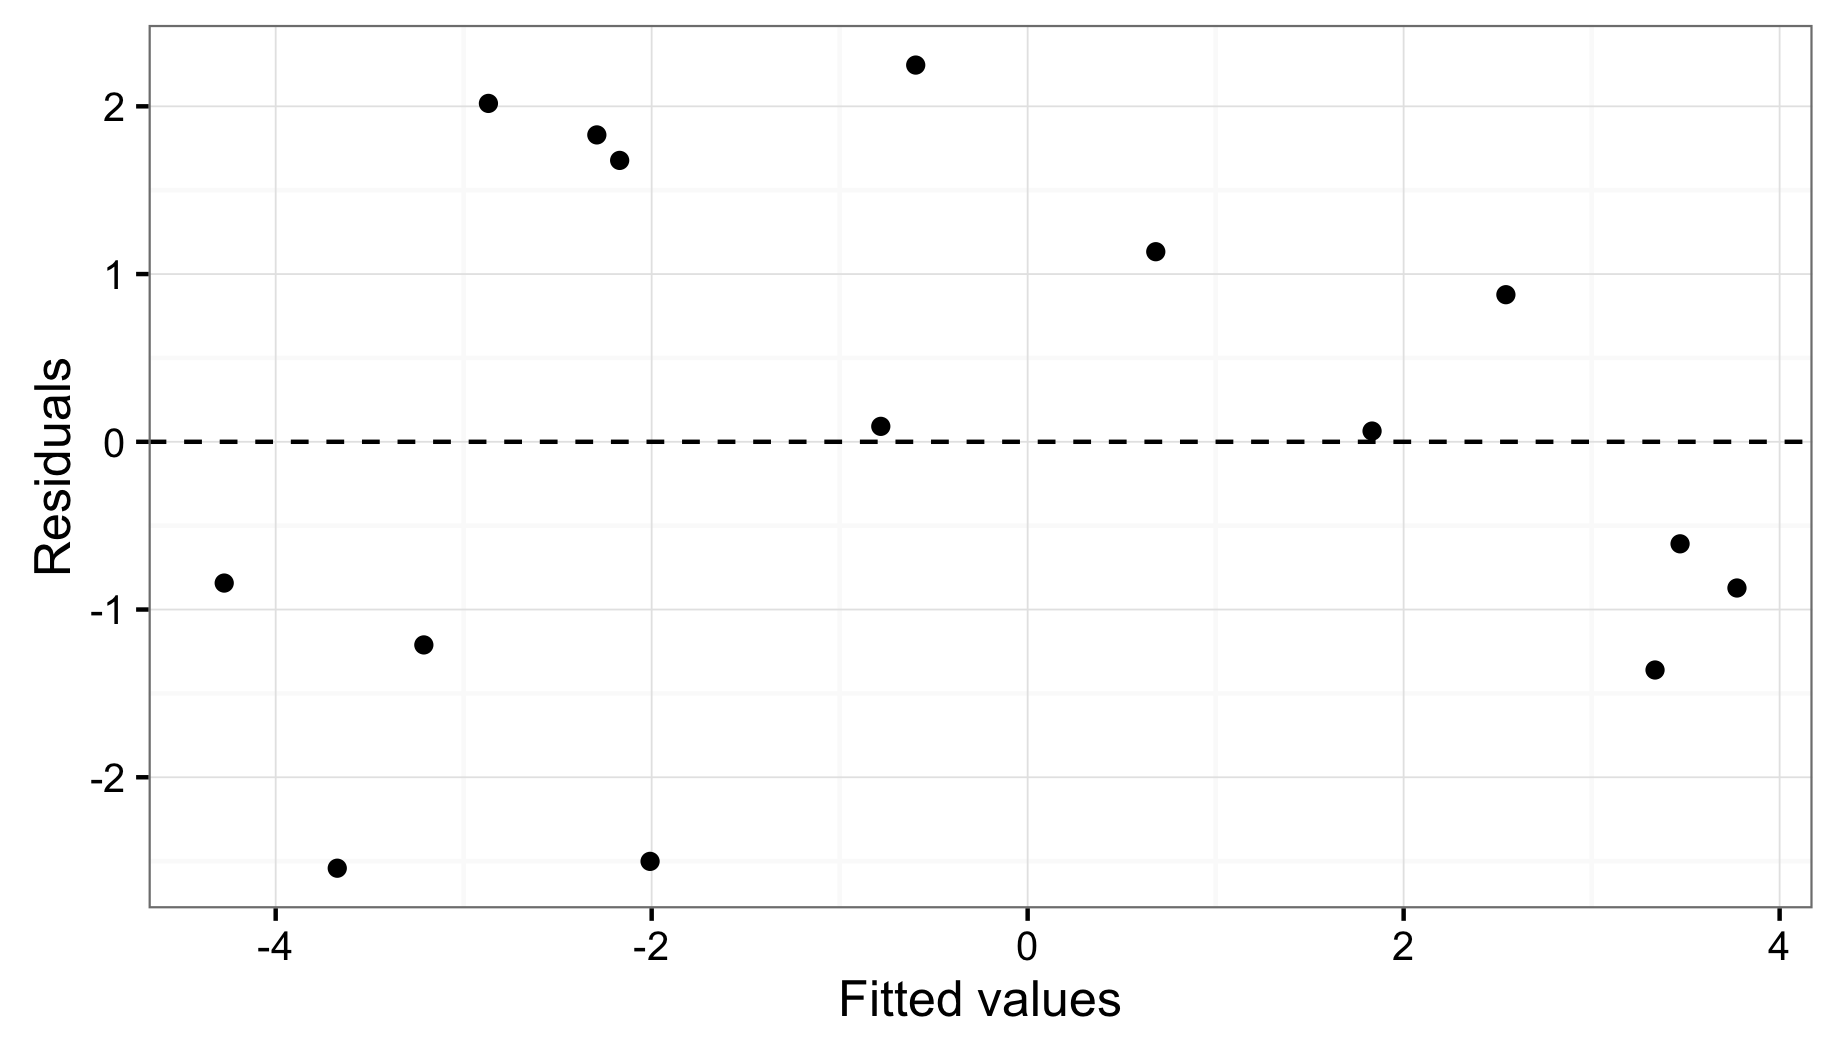
\includegraphics[width=4.25in]{4c.png}
	\caption{Residual plot for the fitted model from part (\ref{prob:0817b}).}
	\label{fig:4c}
\end{figure}

There's no horn-shaped pattern present, but it does appear that even the log-transformed data has some nonlinearity --- the residuals are negative at the extreme values of fitted values, but positive near the center. This suggests that the addition of a $\log(X)^2$ term may be beneficial. The residual plot does not indicate nonconstant variance or the presence of extreme outliers.

\end{parts}


\titledquestion{\ramsey 8.20}

\begin{parts}

\part \textit{Draw a scatterplot of Democratic percentage of absentee ballots versus Democratic percentage of machine-counted ballots. Use a separate plotting symbol to highlight the disputed election.}

A scatterplot of Democratic percentage of absentee ballots versus Democratic percentage of machine-counted ballots is shown in Figure \ref{fig:5a}.

\begin{figure}[!h]
	\centering
	\captionsetup{width=0.8\textwidth}
	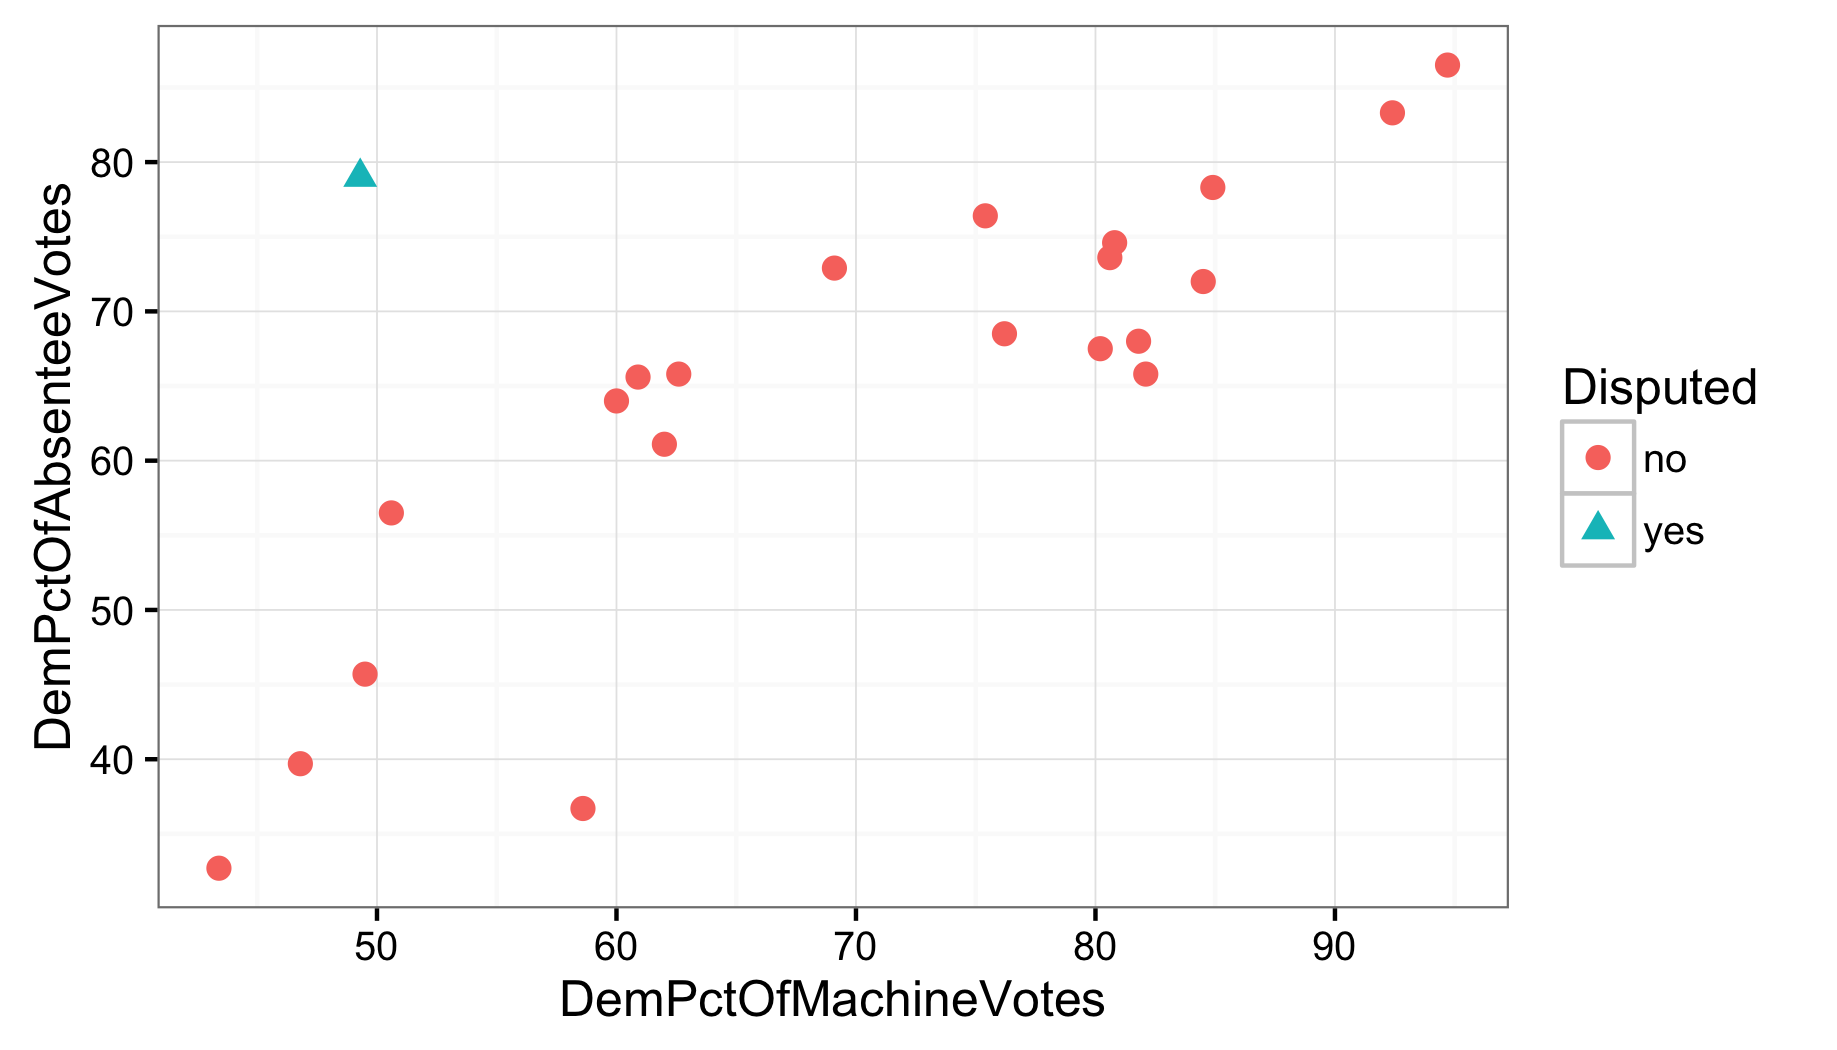
\includegraphics[width=4.25in]{5a.png}
	\caption{Scatterplot of Democratic percentage of absentee ballots versus Democratic percentage of machine-counted ballots. The disputed election is indicated with a blue triangle.}
	\label{fig:5a}
\end{figure}


\part \textit{(i) Fit the simple linear regression of absentee percentage on machine-count percentage, excluding the disputed election. (ii) Draw this line on the scatterplot. Also include a 95\% prediction band. (iii) What does this plot reveal about the unusualness of the absentee percentage in the disputed election?}

A summary of the fitted linear regression on the data excluding the disputed election is shown below.

\begin{codeSmall}
> lmVoteExclDisputed <- lm(formula=DemPctOfAbsenteeVotes~DemPctOfMachineVotes,
+                          data=voteData, subset=(Disputed=="no"))
> summary(lmVoteExclDisputed)

Call:
lm(formula = DemPctOfAbsenteeVotes ~ DemPctOfMachineVotes, data = voteData, 
    subset = (Disputed == "no"))

Residuals:
    Min      1Q  Median      3Q     Max 
-17.988  -5.090   0.459   7.621   9.405 

Coefficients:
                     Estimate Std. Error t value   Pr(>|t|)    
(Intercept)            5.5339     7.7678   0.712      0.485    
DemPctOfMachineVotes   0.8388     0.1080   7.765 0.00000026 ***
---
Signif. codes:  0 ‘***’ 0.001 ‘**’ 0.01 ‘*’ 0.05 ‘.’ 0.1 ‘ ’ 1

Residual standard error: 7.407 on 19 degrees of freedom
Multiple R-squared:  0.7604,	Adjusted R-squared:  0.7478 
F-statistic:  60.3 on 1 and 19 DF,  p-value: 0.00000026
\end{codeSmall}

The linear regression line and a 95\% prediction band are shown in Figure \ref{fig:5b}. The disputed election is far outside the 95\% prediction band, and the plot reveals that the results in the disputed election are fairly unlikely, given the Democratic percentage of machine-counted votes in this election, and given other historical election results.

\begin{figure}[!h]
	\centering
	\captionsetup{width=0.8\textwidth}
	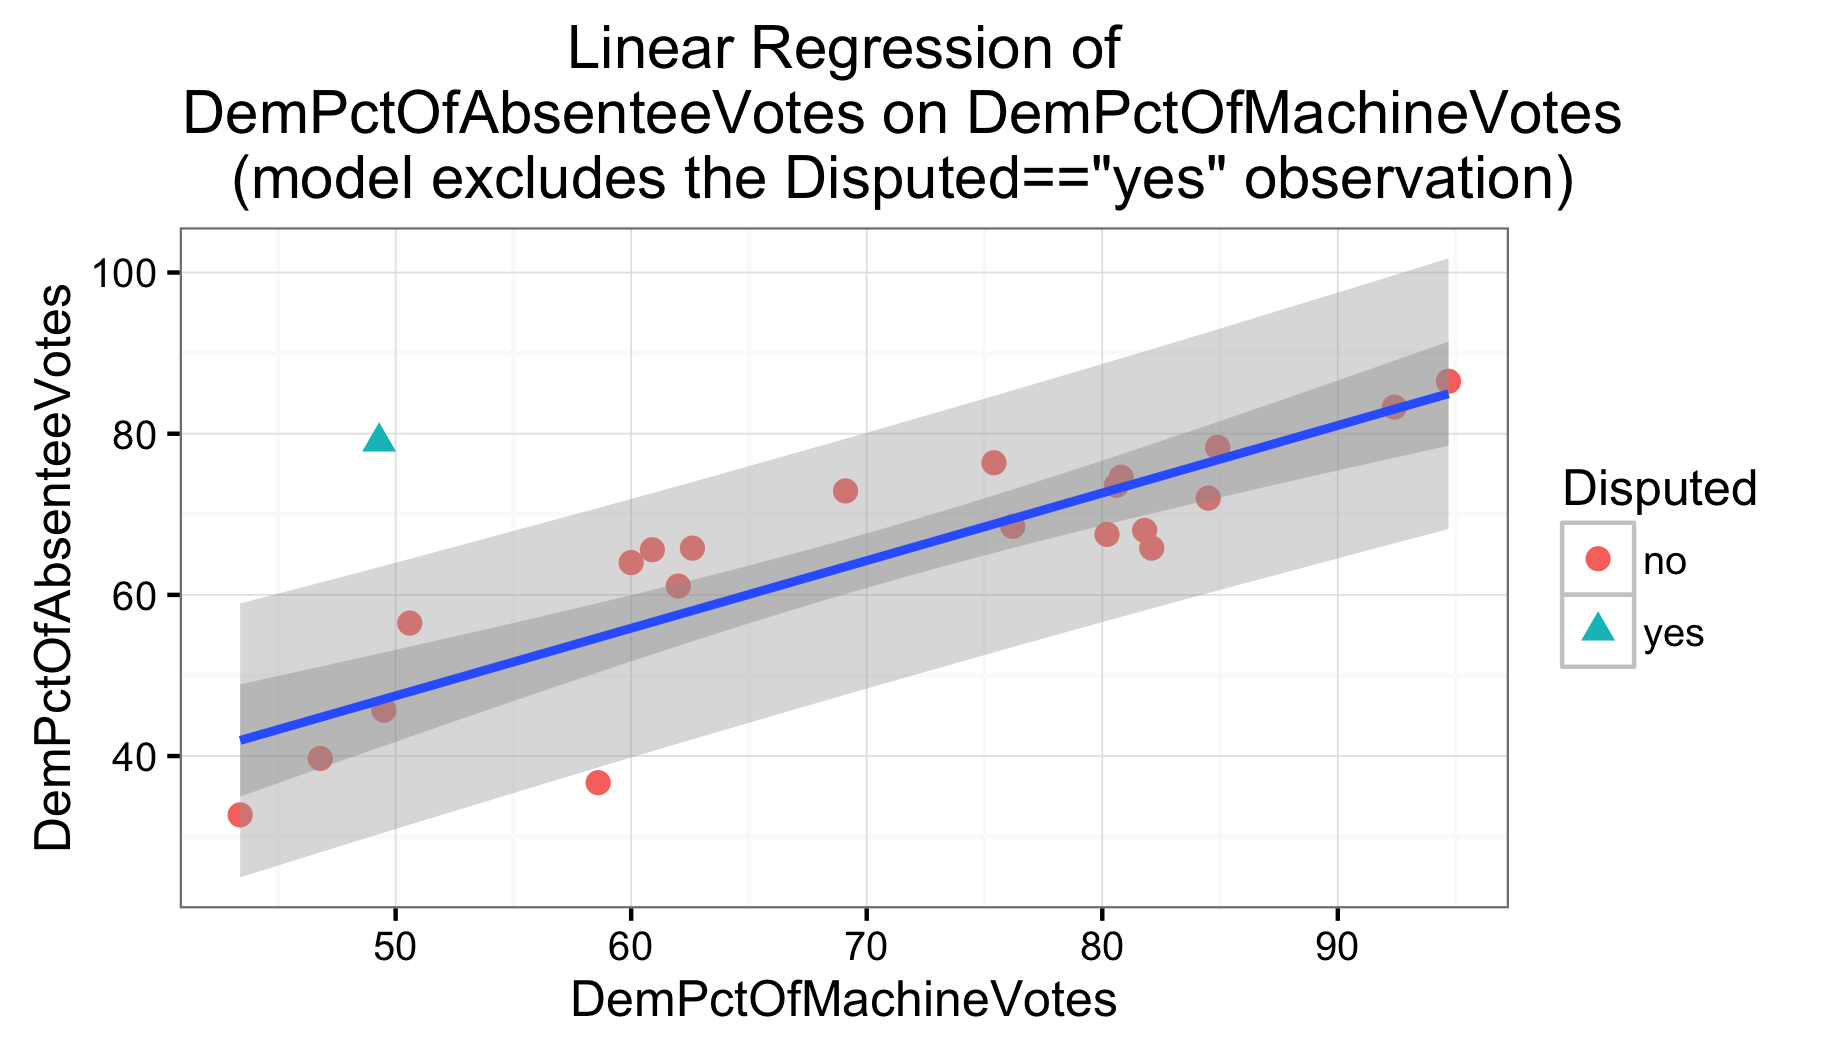
\includegraphics[width=4.25in]{5b.png}
	\caption{Scatterplot of Democratic percentage of absentee ballots versus Democratic percentage of machine-counted ballots. The linear model is constructed using only the undisputed elections. The 95\% prediction band is in light gray, and the 95\% confidence band is in dark gray.}
	\label{fig:5b}
\end{figure}


\part \textit{(i) Find the prediction and standard error of prediction from this fit if the machine-count percentage is 49.3 (as it is for the disputed election). (ii) How many estimated standard deviations is the observed absentee percentage, 79.0, from this predicted value? (iii) Compare this answer to a t-distribution (with degrees of freedom equal to the residual degrees of freedom in the regression fit) to obtain a p-value.} \label{prob:0820c}
\todo{Problem 5c}








\part \textit{Outliers and data snooping. The p-value in (\ref{prob:0820c}) makes sense if the investigation into the 1993 election was prompted by some other reason. Since it was prompted because the absentee percentage seemed too high, however, the p-value in (\ref{prob:0820c}) should be adjusted for data snooping. Adjust the p-value with a Bonferroni correction to account for all 22 residuals that could have been similarly considered.}

\todo{Problem 5d}








\end{parts}


\titledquestion{\ramsey 9.12}
\todo{Problem 6}




\end{questions}

\listoftodos

\end{document}